% Standalone TikZ figure: Larmor precession of the magnetization vector M
% about the static field B0. Built to cropped PDF (print) and SVG (web/epub)
% by the Makefile in this directory.
\documentclass{article}
\usepackage[paperwidth=120cm,paperheight=120cm,margin=10mm]{geometry}
\pagestyle{empty}
\providecommand{\babelsublr}[1]{#1}
\usepackage{tikz}
\usetikzlibrary{arrows.meta}
\begin{document}
\babelsublr{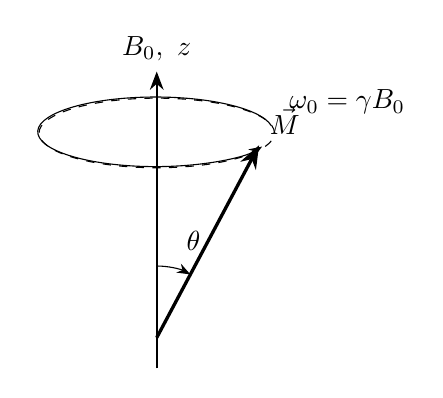
\begin{tikzpicture}[>=Stealth, scale=1.3, line join=round]
  % z-axis / static field B0
  \draw[->, thick] (0,-0.3) -- (0,2.6) node[above] {$B_0,\ z$};
  % precession cone (dashed ellipse traced by the tip of M)
  \draw[dashed] (0,2.0) ellipse (1.15 and 0.34);
  % magnetization vector M
  \draw[->, very thick] (0,0) -- (1.0,1.88) node[above right] {$\vec{M}$};
  % precession sense
  \draw[->] (1.12,2.07) arc (10:335:1.15 and 0.34);
  \node[right] at (1.2,2.3) {$\omega_0 = \gamma B_0$};
  % flip angle annotation
  \draw[->] (0,0.7) arc (90:62:0.7);
  \node at (0.36,0.95) {$\theta$};
\end{tikzpicture}}
\end{document}
